\chapter{Design of oxc scheduling framework\label{chap:design}}

\section{Open-Extension Container Structure\label{sec:design_oxc}}


Linux scheduling is runqueue centered and each scheduling class 
implements a set of interfaces to deal with the runqueue structure.
In mainline Linux, \texttt{struct rq} runqueue is a per CPU structure.
On each CPU, based on its runqueue, a scheduling system is built up.
Different per CPU scheduling systems cooperate
with each other by task migrations depending on specific scheduling class 
and construct the system level scheduling. 
Every scheduling operation works around the runqueue structure: enqueue,
dequeue, etc. 
The idea is that if there is one extra runqueue, each scheduler can still 
use it as scheduling parameter and a scheduling system can be built around 
it. If there are more than one extra runqueues, they can produce a pseudo 
system level scheduling system.   

Here a data structure named Open-Extension Container(OXC) is proposed,
shown in figure\ref{fig:oxc}.
\begin{figure}[htbp]
        \centering
        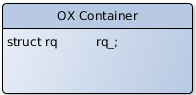
\includegraphics[width=0.5\textwidth]{images/oxc}
        \caption{Open-Extension Container}
        \label{fig:oxc}
\end{figure}
The ox container is designed as an abstract data structure; that is, any data
structure contains a \texttt{struct rq} runqueue inside can be called an ox
container. Now, in the system there is not only per CPU runqueues, but also 
per oxc runqueues.

\section{The oxc scheduling\label{sec:design_oxc_scheduling}}
As ox containers are defined, there are extra runqueues besides per CPU ones 
in a system. For each scheduler, they manage tasks above runqueues according
to implementation details in their scheduling class, and as long as a runqueue
parameter is provided for their schedulinf operations, they have do not care 
it is from a CPU or an ox container.
So as a oxc local runqueue is passed to hooks of scheduling classes, tasks would 
enqueue, operate and dequeue on a per container runqueue. As for tasks and scheduling
classes, there is no difference between a per CPU and per container runqueue.
This can be clearly shown when we see the scheduling scheme in the system 
with oxc scheduling. Recall the path which relates each
task with the per CPU runqueue it runs above in section \ref{sec:LinuxSched_cfs}
and \ref{sec:LinuxSched_rt}. Now let's see the scheduling scheme after the 
ox container joins the system with its local runqueue. 

From figure \ref{fig:oxc_fair_tg} and \ref{fig:oxc_rt_tg} we can see when 
task group scheduling is enabled, the scheduling route we saw before can also
lead a task to its per container runqueue. The same codes can still be used to
find both kinds of runqueues.

\begin{figure}[htbp]
        \centering
        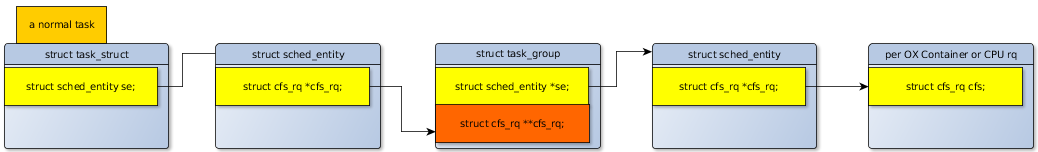
\includegraphics[height=2.5cm, width=\textwidth]{images/cfs_scheduling_scheme_tg_oxc}
        \caption{Scheduling path for normal tasks with fairness grouping}
        \label{fig:oxc_fair_tg}
\end{figure}
\begin{figure}[htbp]
        \centering
        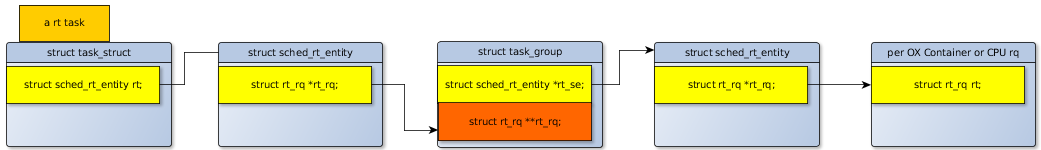
\includegraphics[height=2.5cm, width=\textwidth]{images/rt_scheduling_scheme_tg_oxc}
        \caption{Scheduling path for rt tasks with rt grouping}
        \label{fig:oxc_rt_tg}
\end{figure}

In section \ref{sec:LinuxSched_cfs}, we introduce that when task group
scheduling is not enabled, a macro \texttt{task\_rq} is used to associate
a task to its runqueue. The \texttt{task\_rq} is defined as follows:
\begin{lstlisting}
#define task_rq(p)              cpu_rq(task_cpu(p))
\end{lstlisting}
The macro returns the associated rq for the CPU where the task is currently 
running on. So, when task group scheduling is not enabled, in order to merge
oxc scheduling in the system, a new route to lead a task to a runqueue is 
needed, shown in figure \ref{fig:oxc_task_no_tg}. Actually, this path already 
exists in Linux kernel. Just because in current Linux, there is no runqueue 
other than per CPU ones and people ignore to exploit it.  
\begin{figure}[htbp]
        \centering
        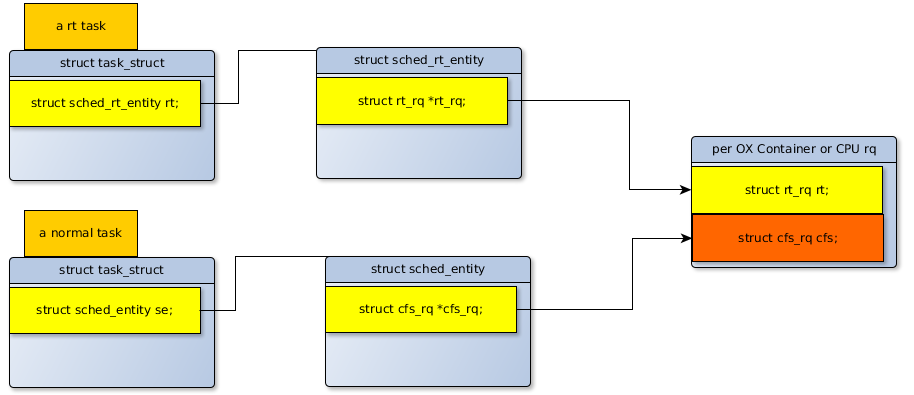
\includegraphics[width=\textwidth]{images/oxc_task_no_tg}
        \caption{New scheduling route for tasks when task group scheduling is not enabled}
        \label{fig:oxc_task_no_tg}
\end{figure}

The first feature of oxc scheduling is that it is compatibe with Linux original
scheduling. Tasks dealt by rt scheduler or cfs can naturally work under the
oxc scheduling system. When there is new scheduling algorithm implemented in
Linux kernel, like the \emph{sched deadline} patch we mentioned before, the
new scheduler has to fullfill details behind scheduling interfaces in 
\texttt{struct sched\_class}. Again, for each shceduling class, they do not
care the interface is passed a per CPU or per container runqueue as the
parameter, and the new scheduling class can also work under oxc scheduling.
So, the ox container structure is open to extension; this is where the name
is from.

Based on per CPU scheduling, each scheduling operation defined in 
\texttt{struct sched\_class} will affect all tasks in the CPU. The
oxc scheduling provides another opportunity to apply a scheduling class in a 
fine grained scale. Now, the scale to apply a scheduler can be controlled 
in the unit of an ox container. 
